\subsection{Query Skeleton Creation}
\label{sec:skeleton}

\todo{why need a skeleton. We divide the whole inference
into three tasks}

In this step, \ourtool performs a simple scan over
the provided input-output examples to capture the basic
structure of the desirable SQL query.

A query skeleton is an incomplete SQL query, consisting
of three basic parts: the table set used in the query, 
the table columns used to join tables, and the table
columns used to project the query results. Besides,
other query parts, such as query conditions and
aggregation operators, are left as unknown and will be
determined later. \todo{the group by columns}

We next describe how \ourtool determines the table set,
joining columns, and projection columns used in a query.



%\item
\vspace{1mm}
{\textbf{Determining the Table Set.}} 
End-users are unwilling to provide more than enough
inputs. Thus, every table in the input example
is expected to be used in the desirable SQL query.
Based on this observation, we assume that every input table
should be used \textit{as least} once in the result query. 
By default, the table set contains all given input tables.
However, it is possible that one input table will be
used for multiple times.
\ourtool does not forbid this case,
rather, it uses a heuristic
to estimate the table set: if the \textit{same} column from
an input table appears more than once in the
example output, we add the input table to the table set the same
number of times.

\todo{we view it as a strong indicator that this table will be joined multiple times and add it to our table
set $T$ using an alias}


%\item
%\vspace{1mm}
%\noindent
{\textbf{Determining Joining Columns. }} Given a set of tables,
there are many ways to join them. Enumerating all possibilities can
introduce a huge number of joining conditions and would quickly
become intractable. To prune the search space, we use
three simple but effective effective rules. 
%based We observe that, in practice, two tables are often joined via the following
%three cases: 
First, tables are often joined on their primary keys with
the same data types, such as joining the \CodeIn{student} table with
the \CodeIn{enrolled} table on the \CodeIn{student\_id} column (Figure~\ref{fig:motivating}).
By contrast, it is unlikely to join two tables with an
Integer column and a String column. Second, tables are often joined
on columns with the same name, such as joining the \CodeIn{student} table
with the \CodeIn{enrolled} table on the
\CodeIn{student\_name} column. Third, it is only meaningful
to join two tables on columns that have the same data type and some
overlapped values. 

\ourtool restricts the search space in uses the above three rules \todo{need to revise}

%It is straightforward to check the first 
%two cases to identify possible joining columns. For the third case, our technique scans the given input tables to check ``value similarity''
%between two arbitrary columns, and selects columns whose ``value similarity'' is above a fixed threshold as joining columns.
\todo{need to implement above.}
\todo{mention how many skeletons will be created}

%\item
%\vspace{1mm}
%\noindent 
{\textbf{Determining Output Columns.}} For each
column in the output table, \ourtool checks whether its name
appears in any of the input table. If so, \ourtool uses
the matched column from the input table as the output column.
to the output column set. Otherwise, the output column
must be produced by using aggregation operators.
\todo{same names}
Consider the example in Figure~\ref{fig:motivating},
\ourtool determines that column {\CodeIn{name}} comes from the \CodeIn{student}
table, while column {\CodeIn{max\_Score}} must be created by using an aggregation operator.
\todo{If there is no column name}
%which the querying result would be projected, our technique checks whether each output
%table column name appears in any input tables. If so, we used the matched column
%from the input table as the output column.  Our technique keeps track of those aggregation columns
%and search for proper aggregates in the next phase (Section~\ref{sec:agg_search}). 
\todo{check the values in the output column}

\todo{It is possible that multiple skeleton can be created. add an algorithm here.}
\vspace{1mm}



\begin{figure}[t]
	\centering
		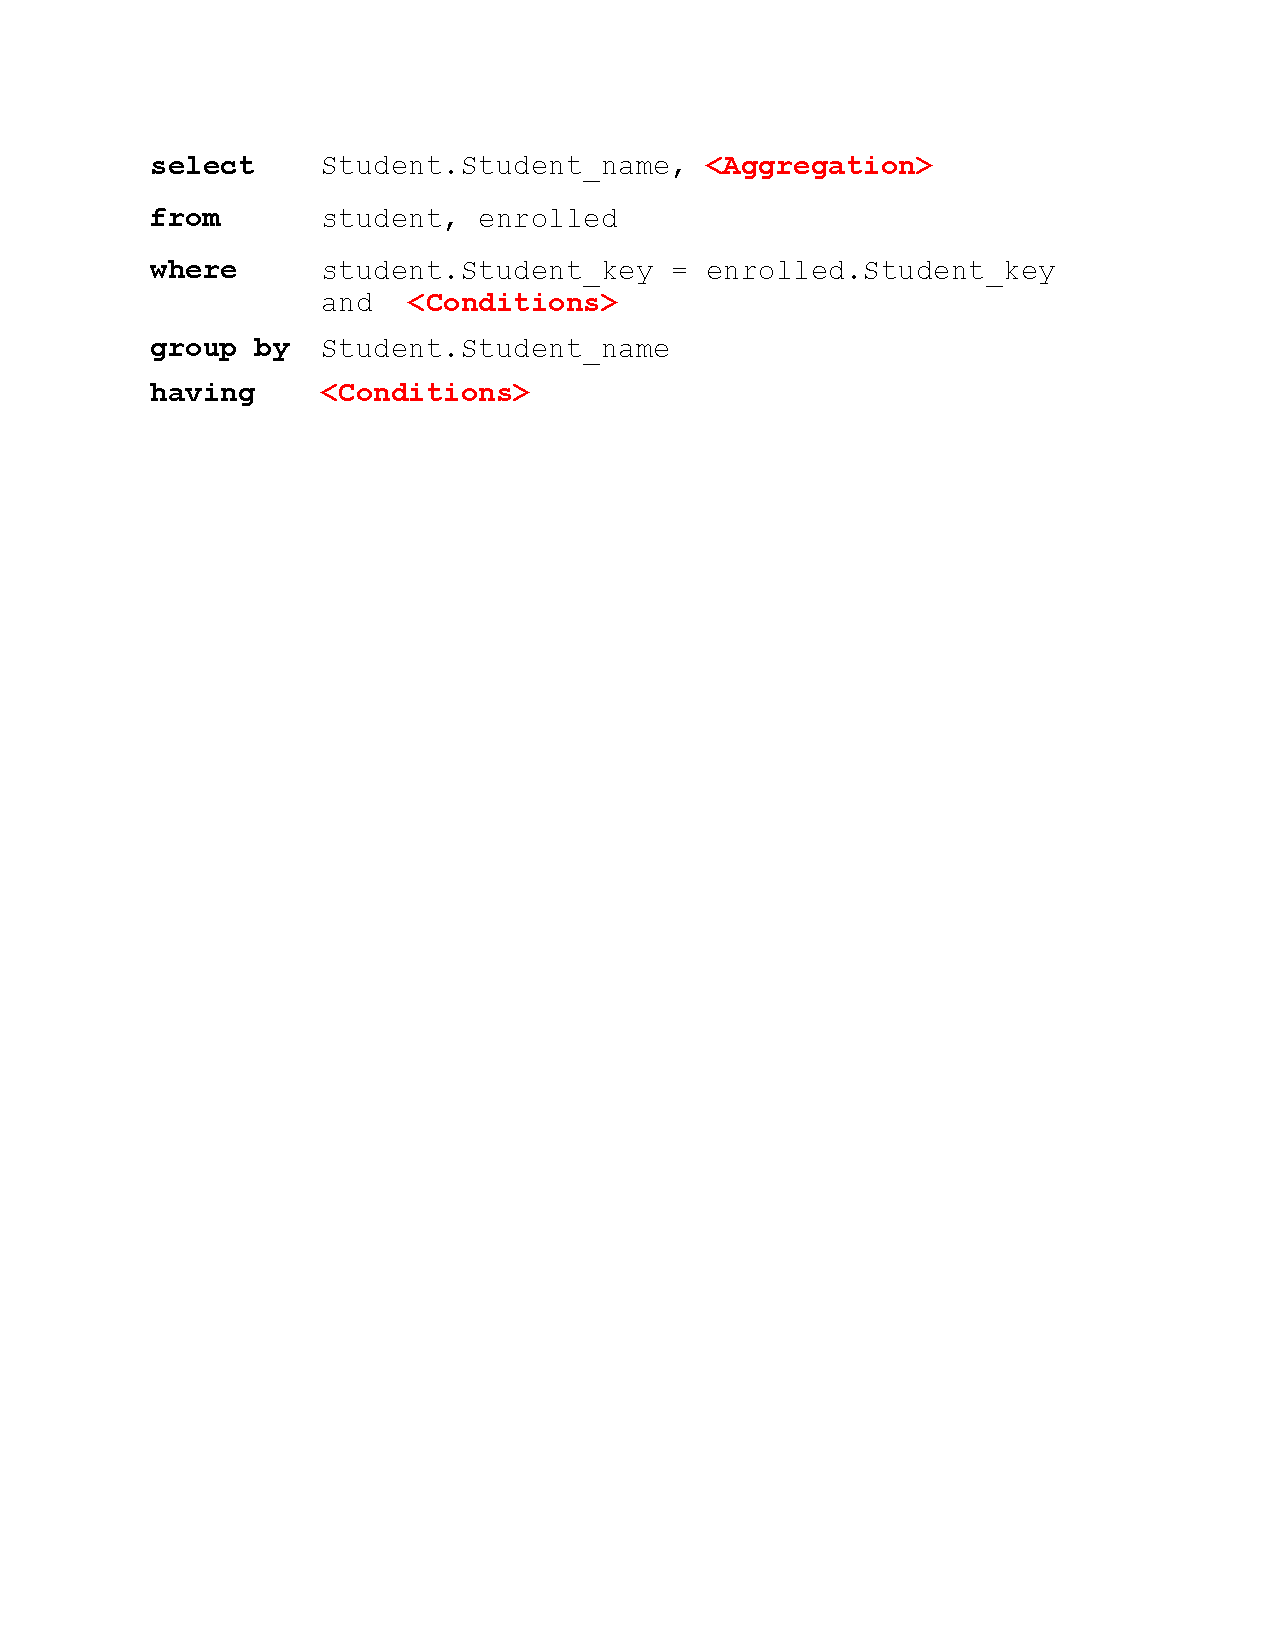
\includegraphics[width=0.45\textwidth]{sql_skeleton.pdf}
	\caption{The SQL skeleton created for the motivating example
in Figure~\ref{fig:motivating}.}
	\label{fig:skeleton}
\end{figure}

Figure~\ref{fig:skeleton} shows the created query skeleton
for the motivating example in Figure~\ref{fig:motivating}.
In this skeleton,  three unknown structures represented by
$<$Aggregation$>$ or $<$Conditions$>$ are in red, and
will be filled in the next phase. \todo{revise text}


\todo{how to create group by}

% which indicates aggregation and group by.

%After determining the table set and joining columns,
%the next step is to identify potential column names on which the result would be projected. If a
%column in the output table  does not appear in any input table's column list, this output column must
%be produced by aggregation. Our algorithm keeps track of these columns and appends a \CodeIn{group by} ... \CodeIn{having} ...
%clause to the query skeleton.

%\end{itemize}

%In summary, this step infers three parts as a query skeleton: tables used in constructing a SQL query, joining conditions
%to connect the input tables, and a list of columns to project the output results.

%It is worth noting that the results obtained from the above steps are not \textit{safe} in
%terms that they may miss some valid SQL queries. 

%We made the above assumption for the sake of tractability,
%since in theory, the bound of table number in a SQL query is $O(n_t!)$, where $n_t$ is the number of given tables;
%while the bound of possible number of join is $O(c_t^2)$ and the bound of the number of conditions is $O(n_t!n_tc_t^2)<O(n_t^3c_t^2)$.

%\subsubsection{Inferring Output Table Schema}

%Lacks schema


%while the bound of possible number of join is $O(c_t^2)$ and the bound of the number of conditions is $O(n_t!n_tc_t^2)<O(n_t^3c_t^2)$.


